Für die erste Messung wird die Schaltung aus Abbildung \ref{fig:schlt1}
aufgebaut.
\begin{figure}[h]
  \centering
  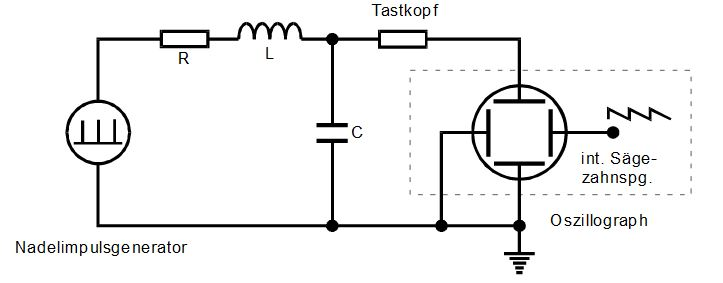
\includegraphics[width=\textwidth]{Bilder/dmpfschalt.JPG}
  \caption{Schaltung für gedämpfte Schwingung\,\cite{354}}
  \label{fig:schlt1}
\end{figure} \\
Mit Hilfe dieses Aufbaus soll der Abfall der Amplitude eines gedämpften
Schwingkreises untersucht werden. Der Nadelimpulsgenerator wird dabei so
eingestellt, dass die Amplitude der Kondensatorspannung $U_\su{C}$ etwa um
den Faktor 3 bis 8 abnimmt. Die Spannung wird am Oszilloskop gegen die Zeit
aufgetragen.
Abbildung \ref{fig:dämpfung} zeigt das ausgegebene Bild des Oszilloskops,
\begin{figure} % Bild kann gerne auch erst in der Auswertung verwendet werden
  \centering
  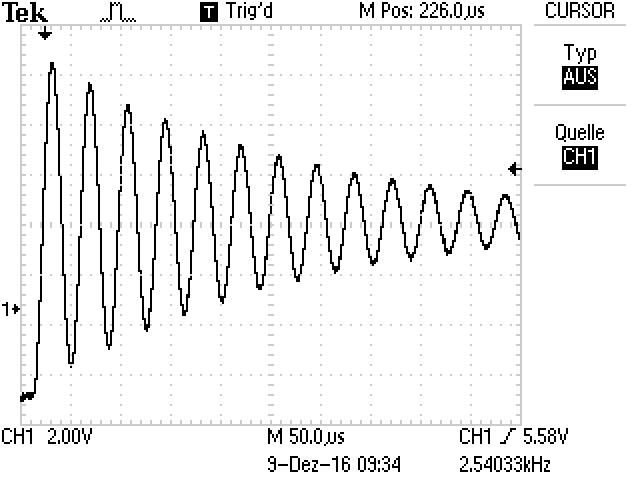
\includegraphics{Bilder/Dmpfung.JPG}
  \caption{Gedämpfte Schwingung am Oszilloskop}
  \label{fig:dämpfung}
\end{figure}
an welchem die Spannungsamplituden mit der zugehörigen Zeitdifferenz $\Delta t$
abgelesen werden. Dazu wird ein Cursor auf die x-Achse gelegt und mit dem anderen Cursor
werden die Hoch- und Tiefpunkte abgefahren. Diese Messung ist relativ genau, da
der dämpfende Einfluss
des Eingangswiderstands des Oszilloskops mit Hilfe des hochohmigen Tastkopfes
($R_\su{i}=10\,\si{\mega\ohm}$) vernachlässigbar klein gehalten wird.
Zur Messung des Widerstands $R_\su{ap}$ wird die Schaltung aus Abbildung
\ref{fig:rapschlt} aufgebaut. \\
\begin{figure}[h]
  \centering
  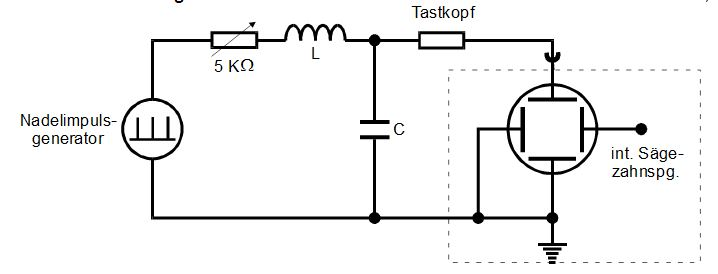
\includegraphics[width=\textwidth]{Bilder/RapSchalt.JPG}
  \caption{Schaltung zur Bestimmung von $R_\su{ap}$\,\cite{354}}
  \label{fig:rapschlt}
\end{figure}
Im Gegensatz zur ersten Messung wird hier ein regulierbarer Widerstand verwendet.
Dieser wird zunächst auf seinen Maximalwert eingestellt, sodass ein Bild
für das Relaxionsverhalten am Oszilloskop angezeigt wird. Dann wird der
Widerstand kontinuierlich verringert, bis ein Überschwingen wie in
Abbildung \ref{fig:aperid} zu sehen ist.
\begin{figure}[h]
  \centering
  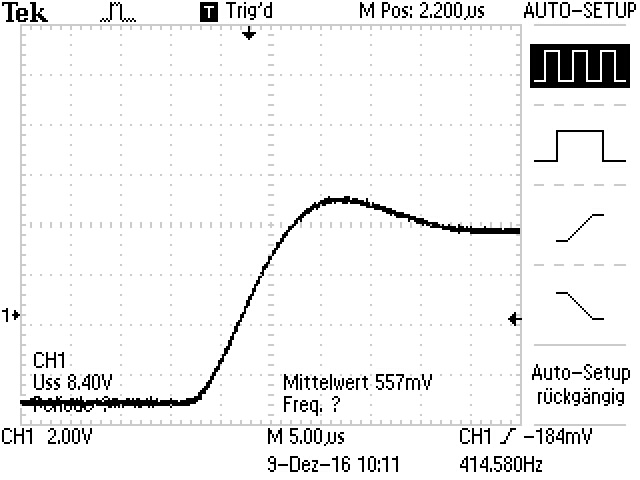
\includegraphics{Bilder/aperid.JPG}
  \caption{Überschwingen der Spannung}
  \label{fig:aperid}
\end{figure} \\
Diesen Zustand bezeichnet man auch als Schwingfall. Der Widerstand soll nun
wieder erhöht werden, bis das Überschwingen gerade verschwindet. Der eingestellte
Widerstand wird als $R_\su{ap}$ notiert.
\newpage
Als nächstes wird die Frequenzabhängigkeit der Kondensatorspannung untersucht.
Hierfür wird die Schaltung aus Abbildung \ref{fig:phaseschlt} aufgebaut.
\begin{figure}[h]
  \centering
  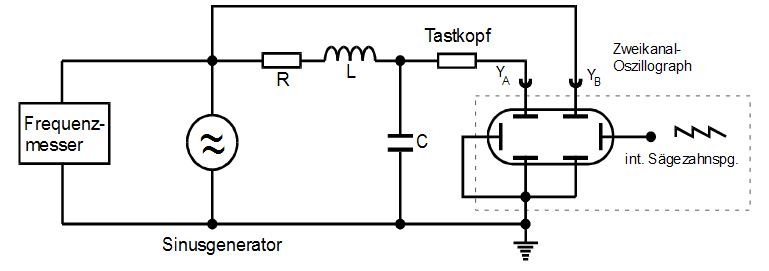
\includegraphics[width=\textwidth]{Bilder/Phaseschalt.JPG}
  \caption{RCL-Schwingkreis zur Untersuchung der Kondensatorspannung\,\cite{354}}
  \label{fig:phaseschlt}
\end{figure}
Zunächst wird die Erregerspannung $U$ gemessen und notiert. Die Frequenz $\nu$
wird nun von $(15-50)\kHz$ in $5\kHz$ Schritten variiert und die dazugehörigen
Werte für die Spannung notiert. Ziel hierbei ist es, die Frequenz für die
Maximalspannung herauszufinden. Die Frequenz, bei der die Spannung maximal wird,
wird auch als Resonanzfrequenz $U_\su{res}$ bezeichnet. Für eine genauere
Auswertung wird der Bereich $\pm 5\kHz$ um das Spannungsmaximum erneut mit $1\kHz$
Schritten gemessen.
Abschließend soll die Phasenverschiebung $\Delta\varphi$ zwischen
Kondensator- und Erregerspannung in Abhängigkeit der Frequenz
bestimmt werden. Es wird weiterhin der Aufbau aus Abbildung
\ref{fig:phaseschlt} verwendet. Beide Spannungsverläufe werden übereinander
angezeigt, sodass sich ein Bild wie in Abbildung \ref{fig:dphi} ergibt. Die
Frequenz wird nun wie zuvor von $(15-50)\kHz$ variiert. Der zeitliche Abstand
der Hochpunkte wird mit der Cursorfunktion des Oszilloskops gemessen. Die
Periodendauer kann hierbei über die Frequenz berechnet werden und muss nicht
explizit gemessen werden. Die Phasenverschiebung ergibt sich mittels
\begin{equation}
  \Delta\varphi_\su{rad} = 2\pi \cdot \nu \cdot \Delta t
\end{equation}
aus den gemessenen $\Delta t$ Werten.
\begin{figure}
  \centering
  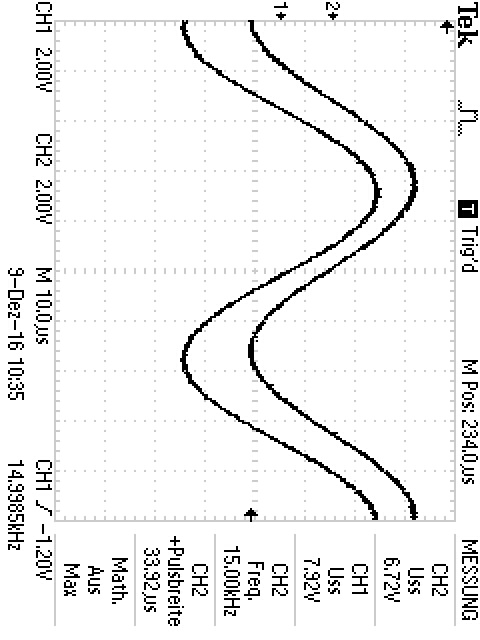
\includegraphics[angle=90]{Bilder/dphi.JPG}
  \caption{Darstellung der Phasenverschiebung am Oszilloskop}
  \label{fig:dphi}
\end{figure}
